\begin{subsectionframemod}{Difference between Natural and Aerial Images}
    \begin{figure}[!h]
    \centering
    \begin{tabular}{cc}
        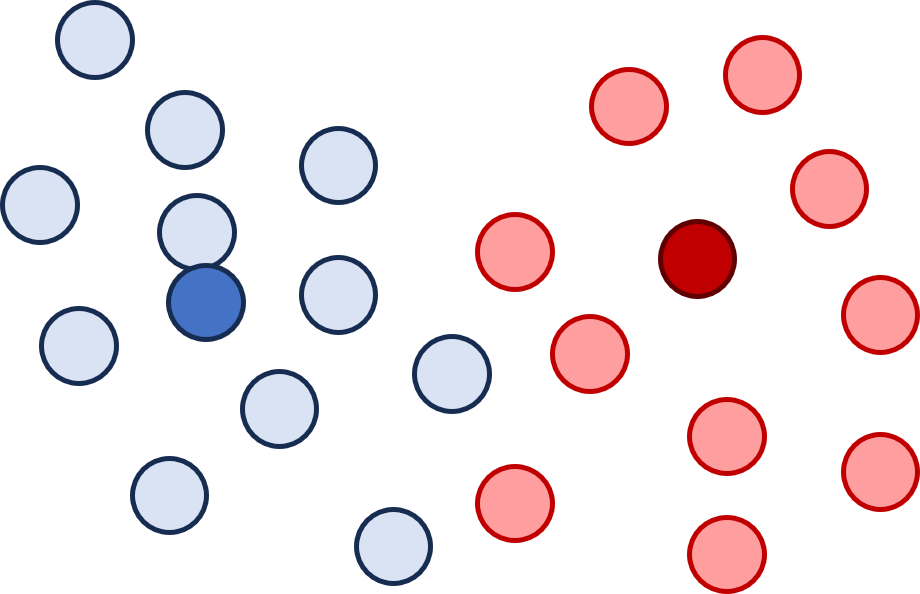
\includegraphics[scale=0.25]{Figures/con_sep} &
        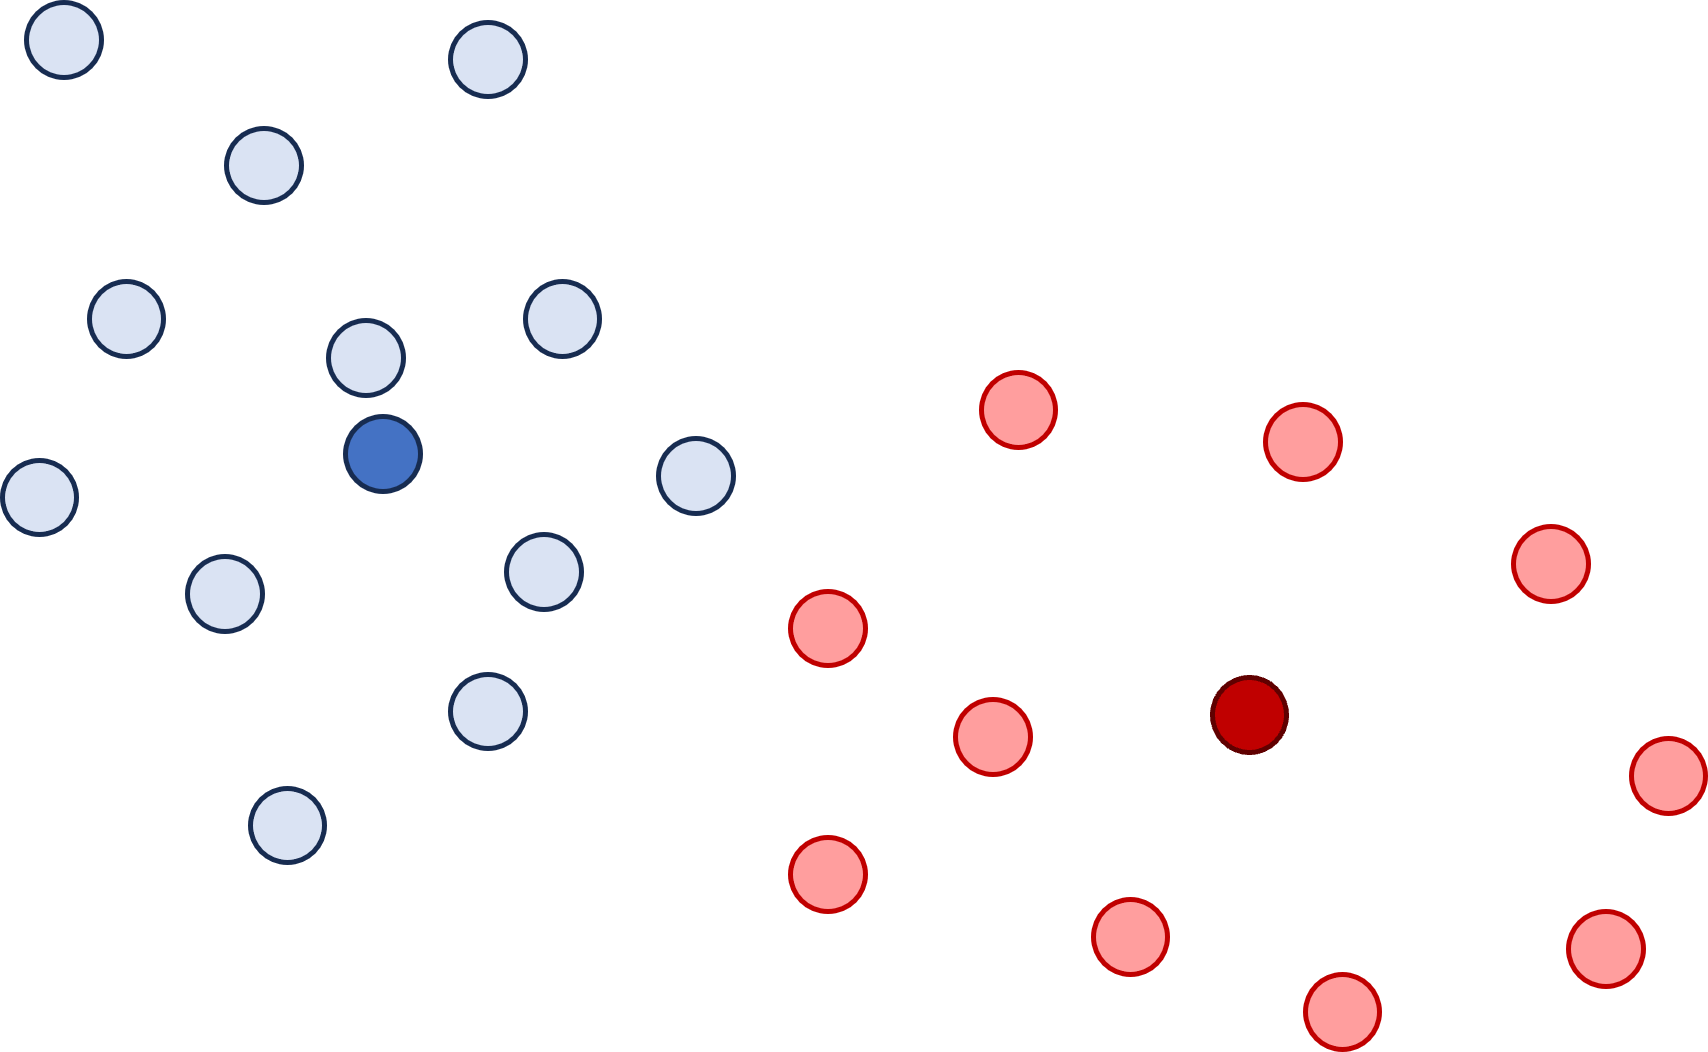
\includegraphics[scale=0.25]{Figures/ncon_sep} \\
        (a) Variance intra-classe faible, & (b) Variance intra-classe forte,\\
         Variance inter-classe forte, & Variance inter-classe forte, \\
         \\
        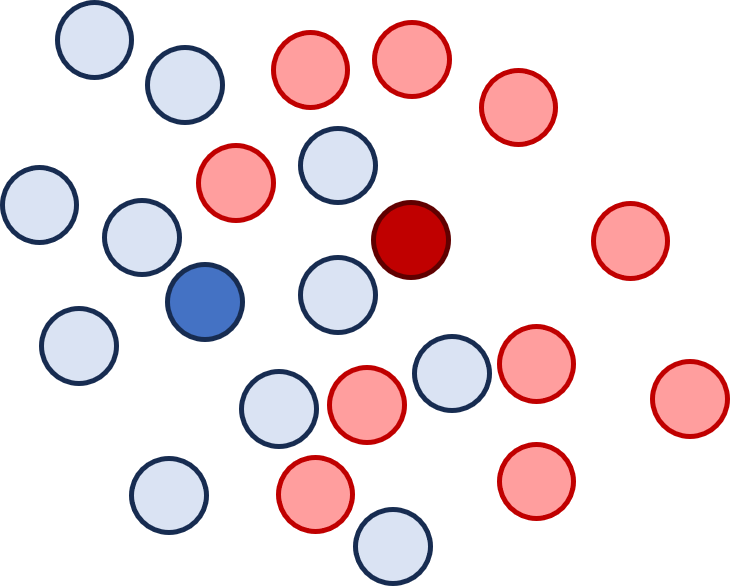
\includegraphics[scale=0.25]{Figures/con_nsep} &
        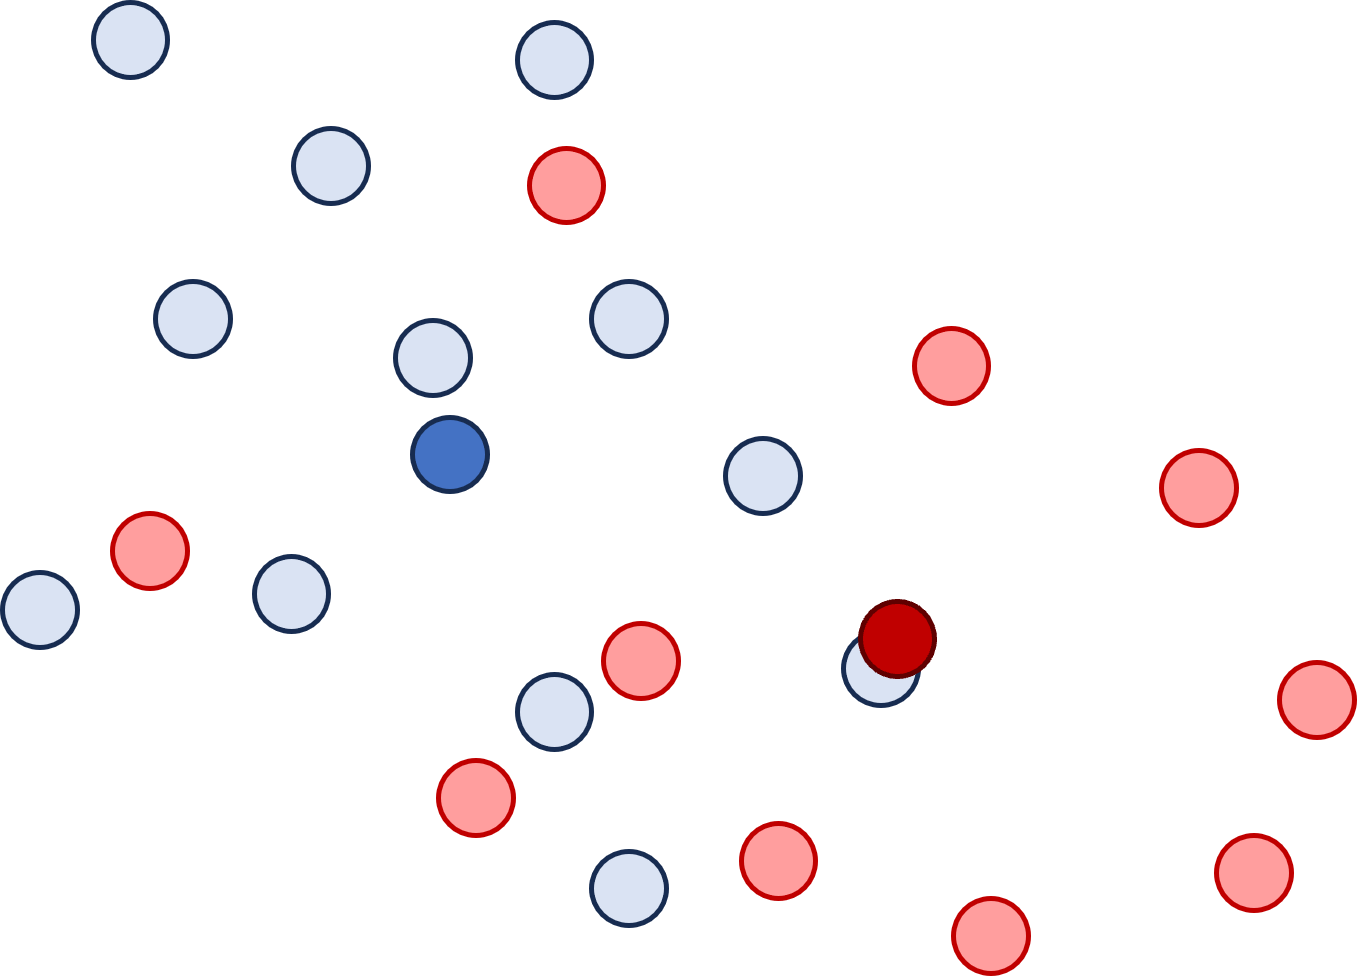
\includegraphics[scale=0.25]{Figures/ncon_nsep}\\
        (d) Variance intra-classe faible, & (c) Variance intra-classe forte, \\
        Variance inter-classe faible,  & Variance inter-classe faible, \\
    \end{tabular}
    \caption{Illustration conceptuelle de la séparabilité des classes en relation avec les variances inter-classes et intra-classes. Les projections dans l'espace latent des images d'une classe sont représentées par des points bleus, tandis que les projections d'une autre classe sont marquées en rouge, avec les barycentres de chaque classe indiqués par des points plus foncés.}
    \label{fig:sep_classes}
\end{figure}
\end{subsectionframemod}



